% vim:fdm=marker
\documentclass[final,t]{beamer}

% Packages and Title %{{{
%\usepackage[orientation=landscape,size=a0,scale=1.4,debug]{beamerposter}
\usepackage[orientation=landscape,size=custom,width=148.625,height=105.125,scale=1.75,debug]{beamerposter}
\usetheme{FusionASU}
\usepackage{amssymb}
\usepackage{amsfonts}
\usepackage{amsmath}
\usepackage{mathtools}
\usepackage{lipsum}
\usepackage{xfrac}
\usepackage{soul}
\usepackage{setspace}
\usepackage{float}
\usepackage{calc,ifthen}
\usepackage{epsfig}
\usepackage[normalem]{ulem} 
\usepackage{xr}
\bibliographystyle{pnas}

\usepackage{amssymb,amsfonts,amsmath}

% references
\usepackage[bibstyle=authoryear, citestyle=authoryear-comp,hyperref=auto]{biblatex}
\bibliography{references}

\definecolor{tangocolordarkchameleon}{HTML}{4E9A06}
\definecolor{tangocolordarkscarletred}{HTML}{CE5C00}
\definecolor{boiseblue}{RGB}{31,65,155}

\renewcommand{\topfraction}{1}             	% PLEASE DO NOT REMOVE THESE COMMANDS:
\renewcommand{\dbltopfraction}{1}          	% THE FIGURES GET PLACED AWFULLY WITHOUT
\renewcommand{\bottomfraction}{1}          % THEM!!
\renewcommand{\textfraction}{0}
\newcommand{\rep}[2]{\sout{#1} \textcolor{red}{#2}}

\nonstopmode

% document properties
\title{Can a double-stranded DNA function as \\ \vskip0.5ex the simplest and fastest biomolecular rotary motor}
\author{\textcolor{boiseblue}{\vskip0.5ex Franky Djutanta$^{a}$, Bernard Yurke$^{b}$ \textrm{\textit{\&}}  Rizal F. Hariadi$^{c}$\\
\vskip0.75ex {\small $^{a}$The Biodesign Institute, Arizona State University, $^{b}$Department of Physics, Boise State University,\\ $^{c}$Department of Physics \textrm{\textit{\&}} the Biodesign Institute, Arizona State University.}}}
\institute{\ }
%}}}

\begin{document}
\begin{frame}{}
\begin{columns}[t]

% ===== Column 1 ===== {{{
\begin{column}{.28\linewidth}\vskip -0.5ex

\begin{block}{Motivation and background} % {{{
\begin{enumerate}
\item Molecular rotary motors are essential for living system. Examples: F$_0$F$_1$-ATP synthase (max. speed at 4 Hz) and flagellar motor of bactery (max. speed at 100 Hz)$^1$
\begin{columns}
\hskip4.5ex\begin{column}{.5\linewidth}
\begin{figure}
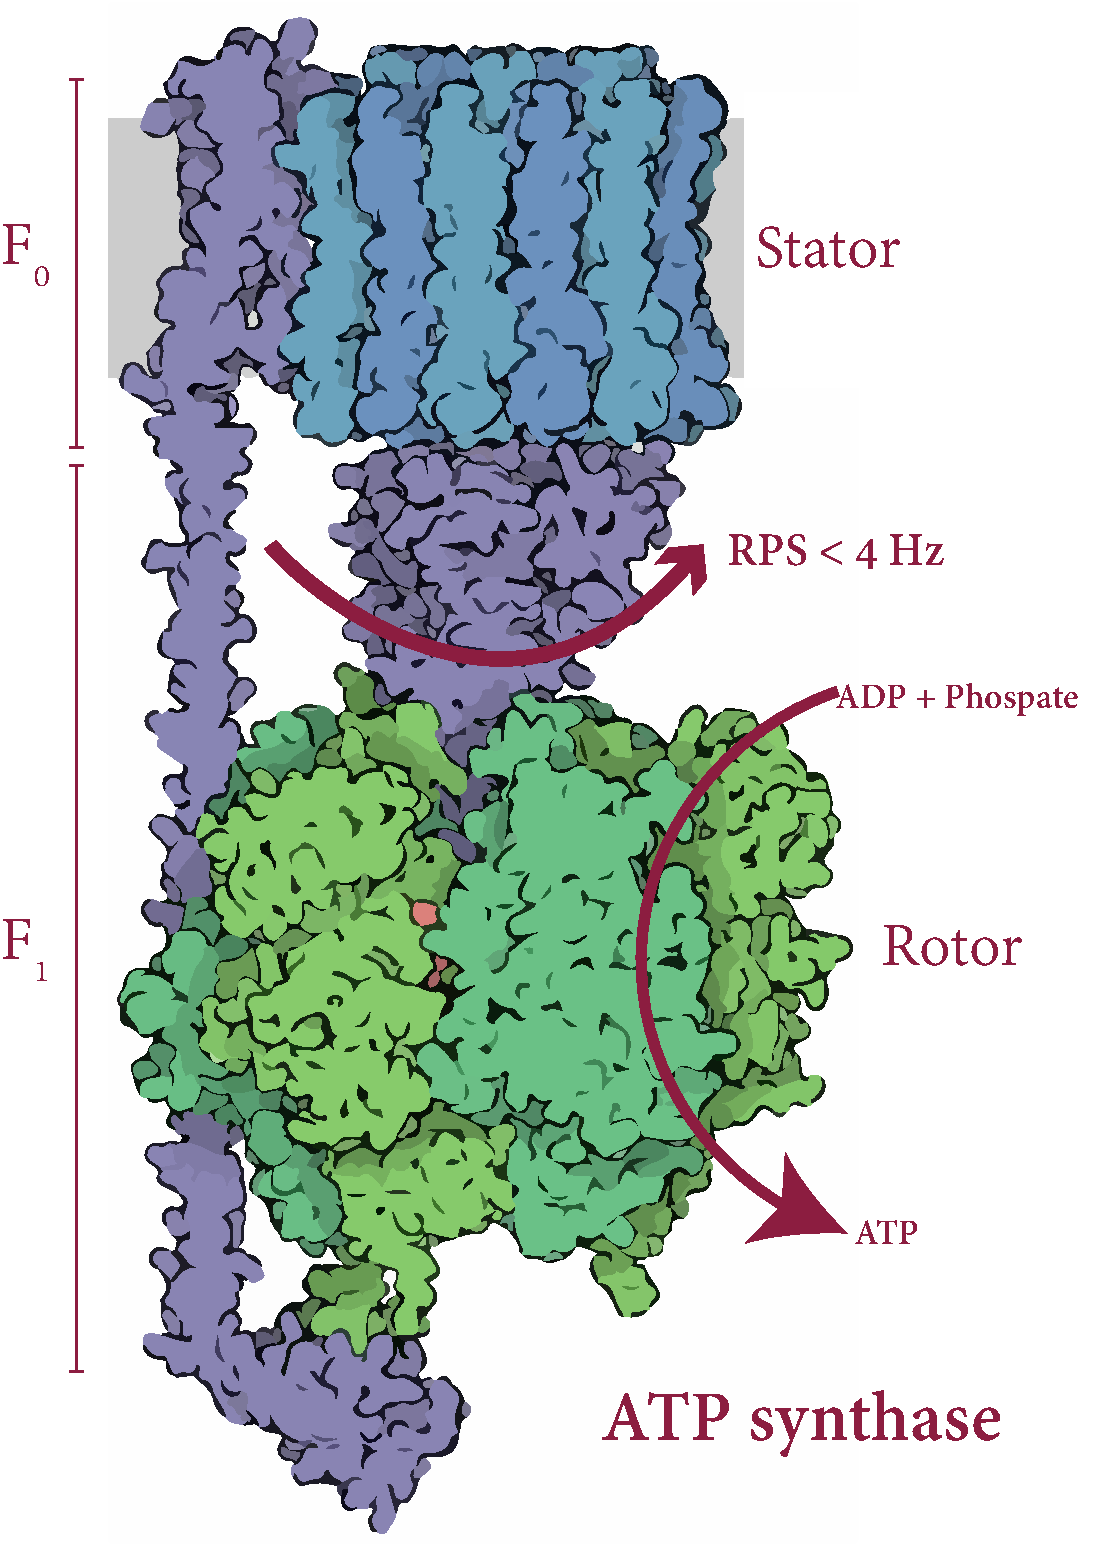
\includegraphics[width=0.99\textwidth]{./f0f1}
\end{figure}
\end{column}

\begin{column}{.4\linewidth}
\begin{figure}
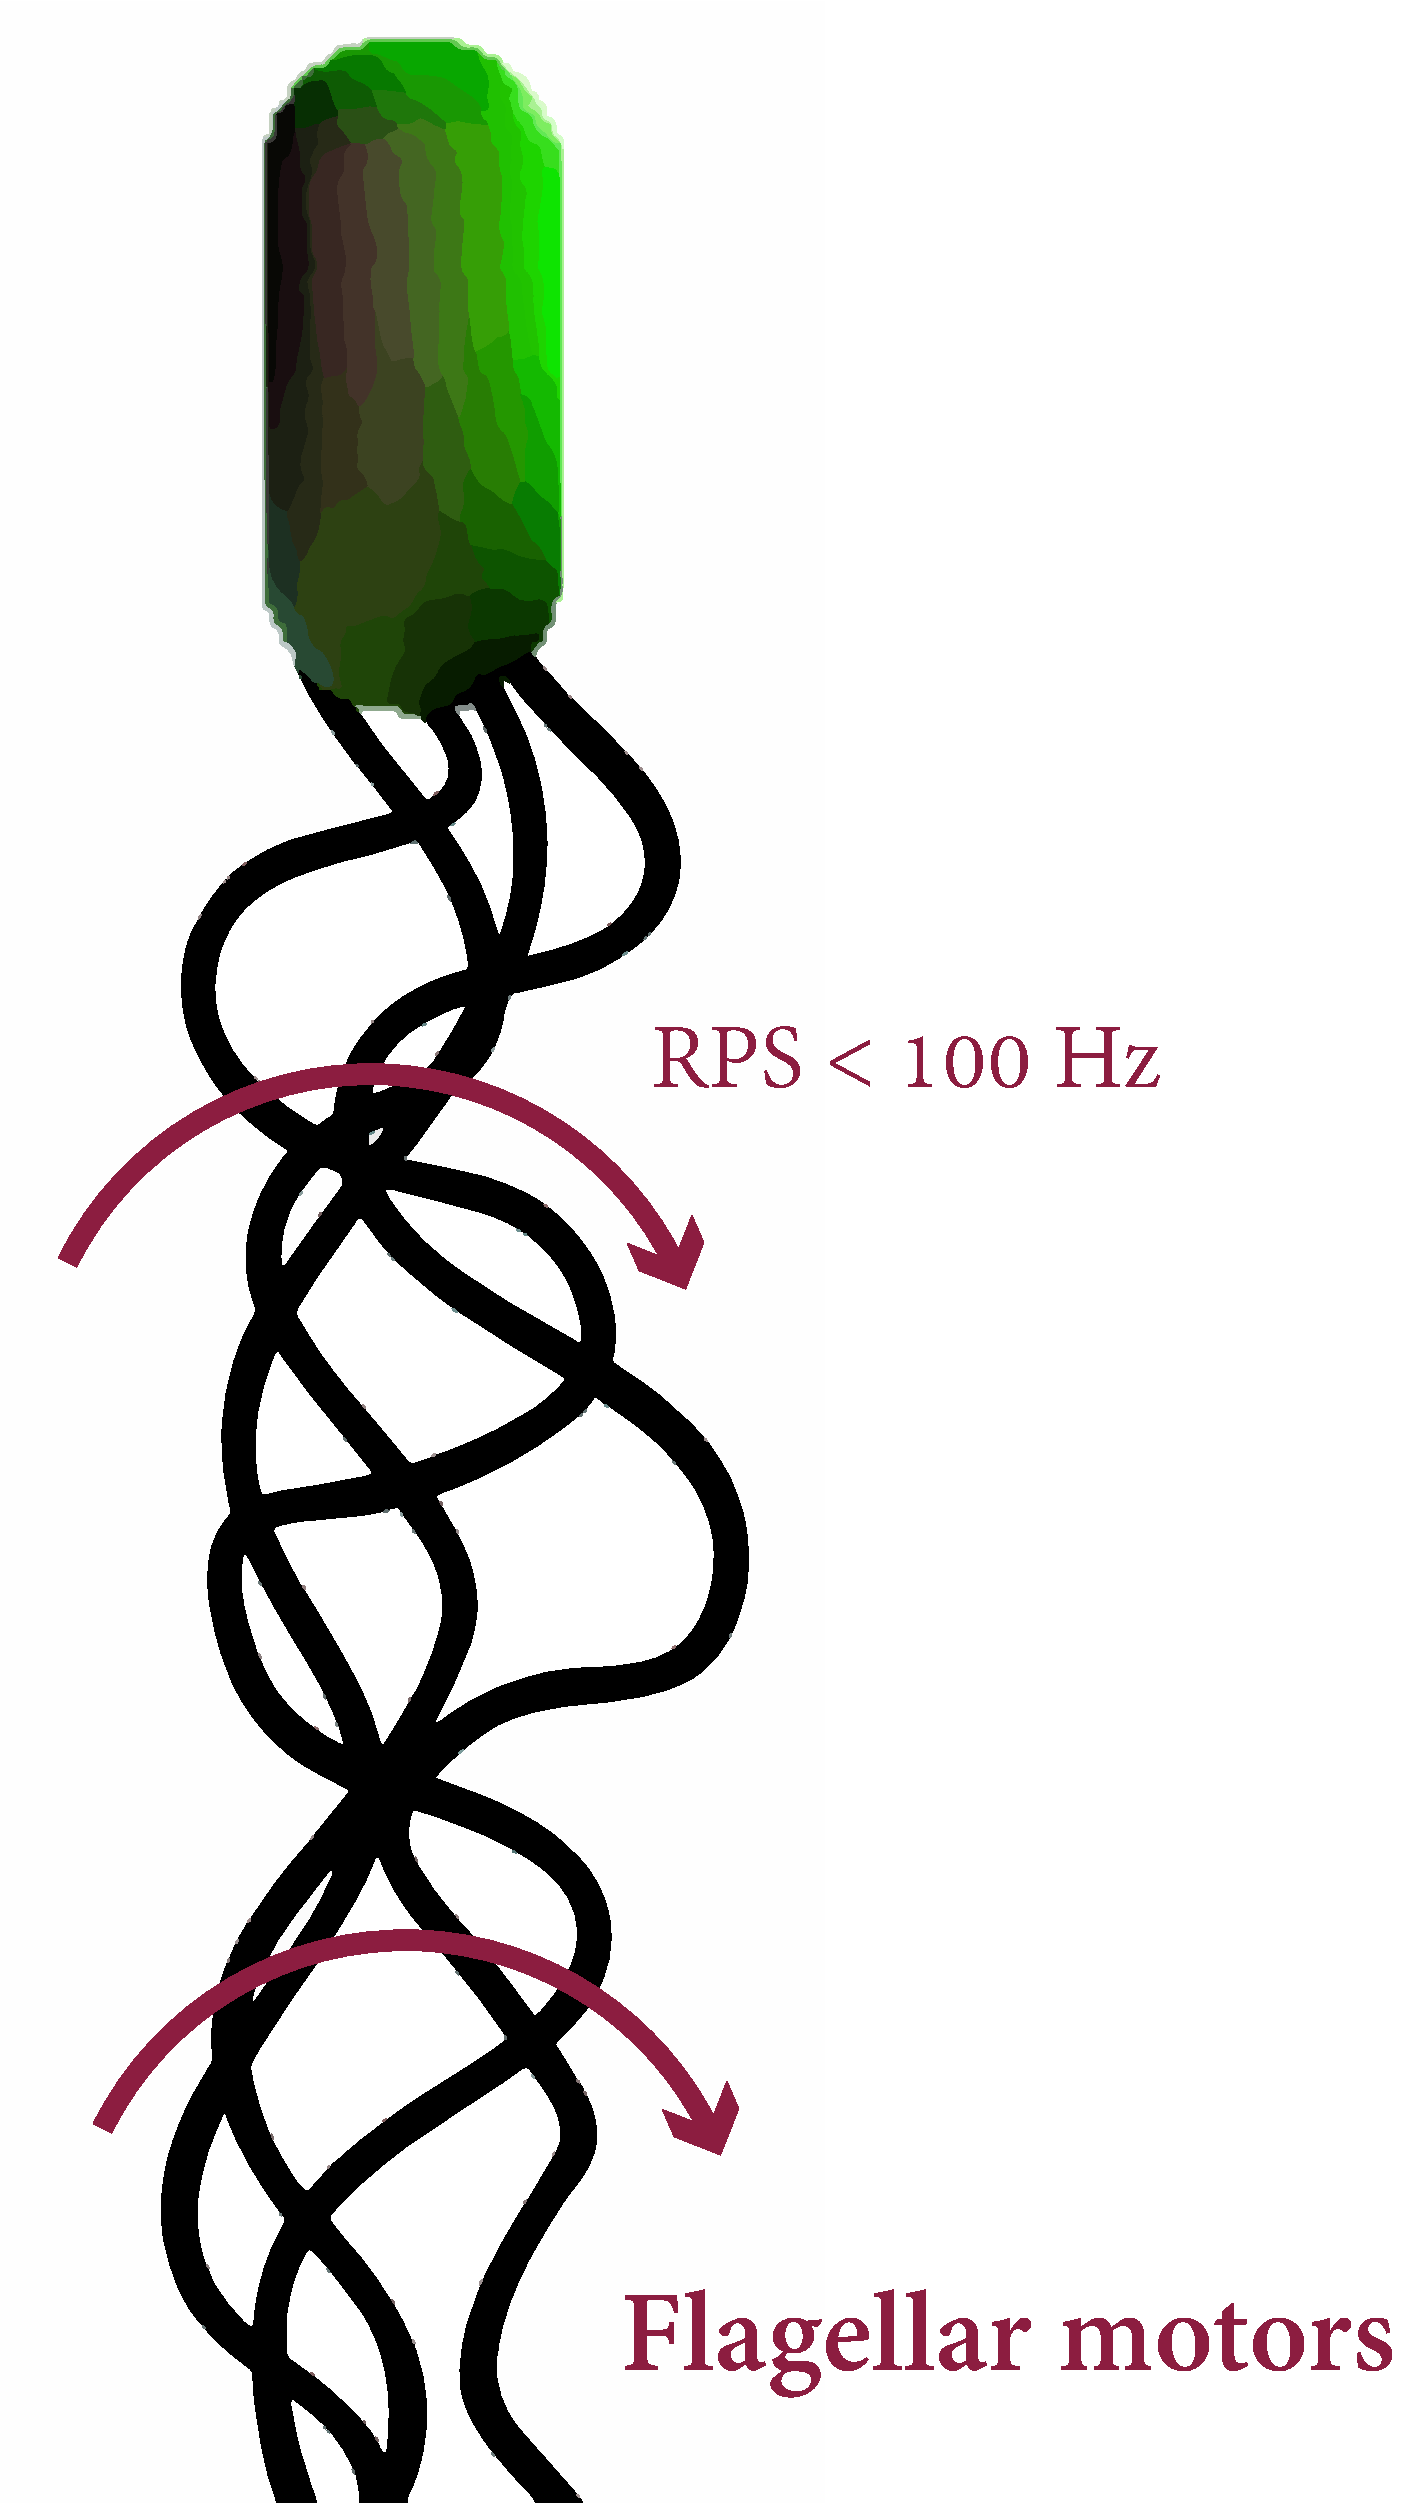
\includegraphics[width=0.9\textwidth]{./flagella}
\end{figure}
\end{column}
\end{columns}

\vskip3.0ex
\item The fastest synthetic biomolecular motor is at 0.005 Hz rotation speed$^2$. 
\begin{columns}
\begin{column}{.4\linewidth}
\vskip1.8ex\begin{figure}
\hskip-5.0ex\includegraphics[width=0.9\textwidth]{./nobel}
\end{figure}
\end{column}

\begin{column}{.4\linewidth}
\vskip1.8ex\begin{figure}
\hskip-5.0ex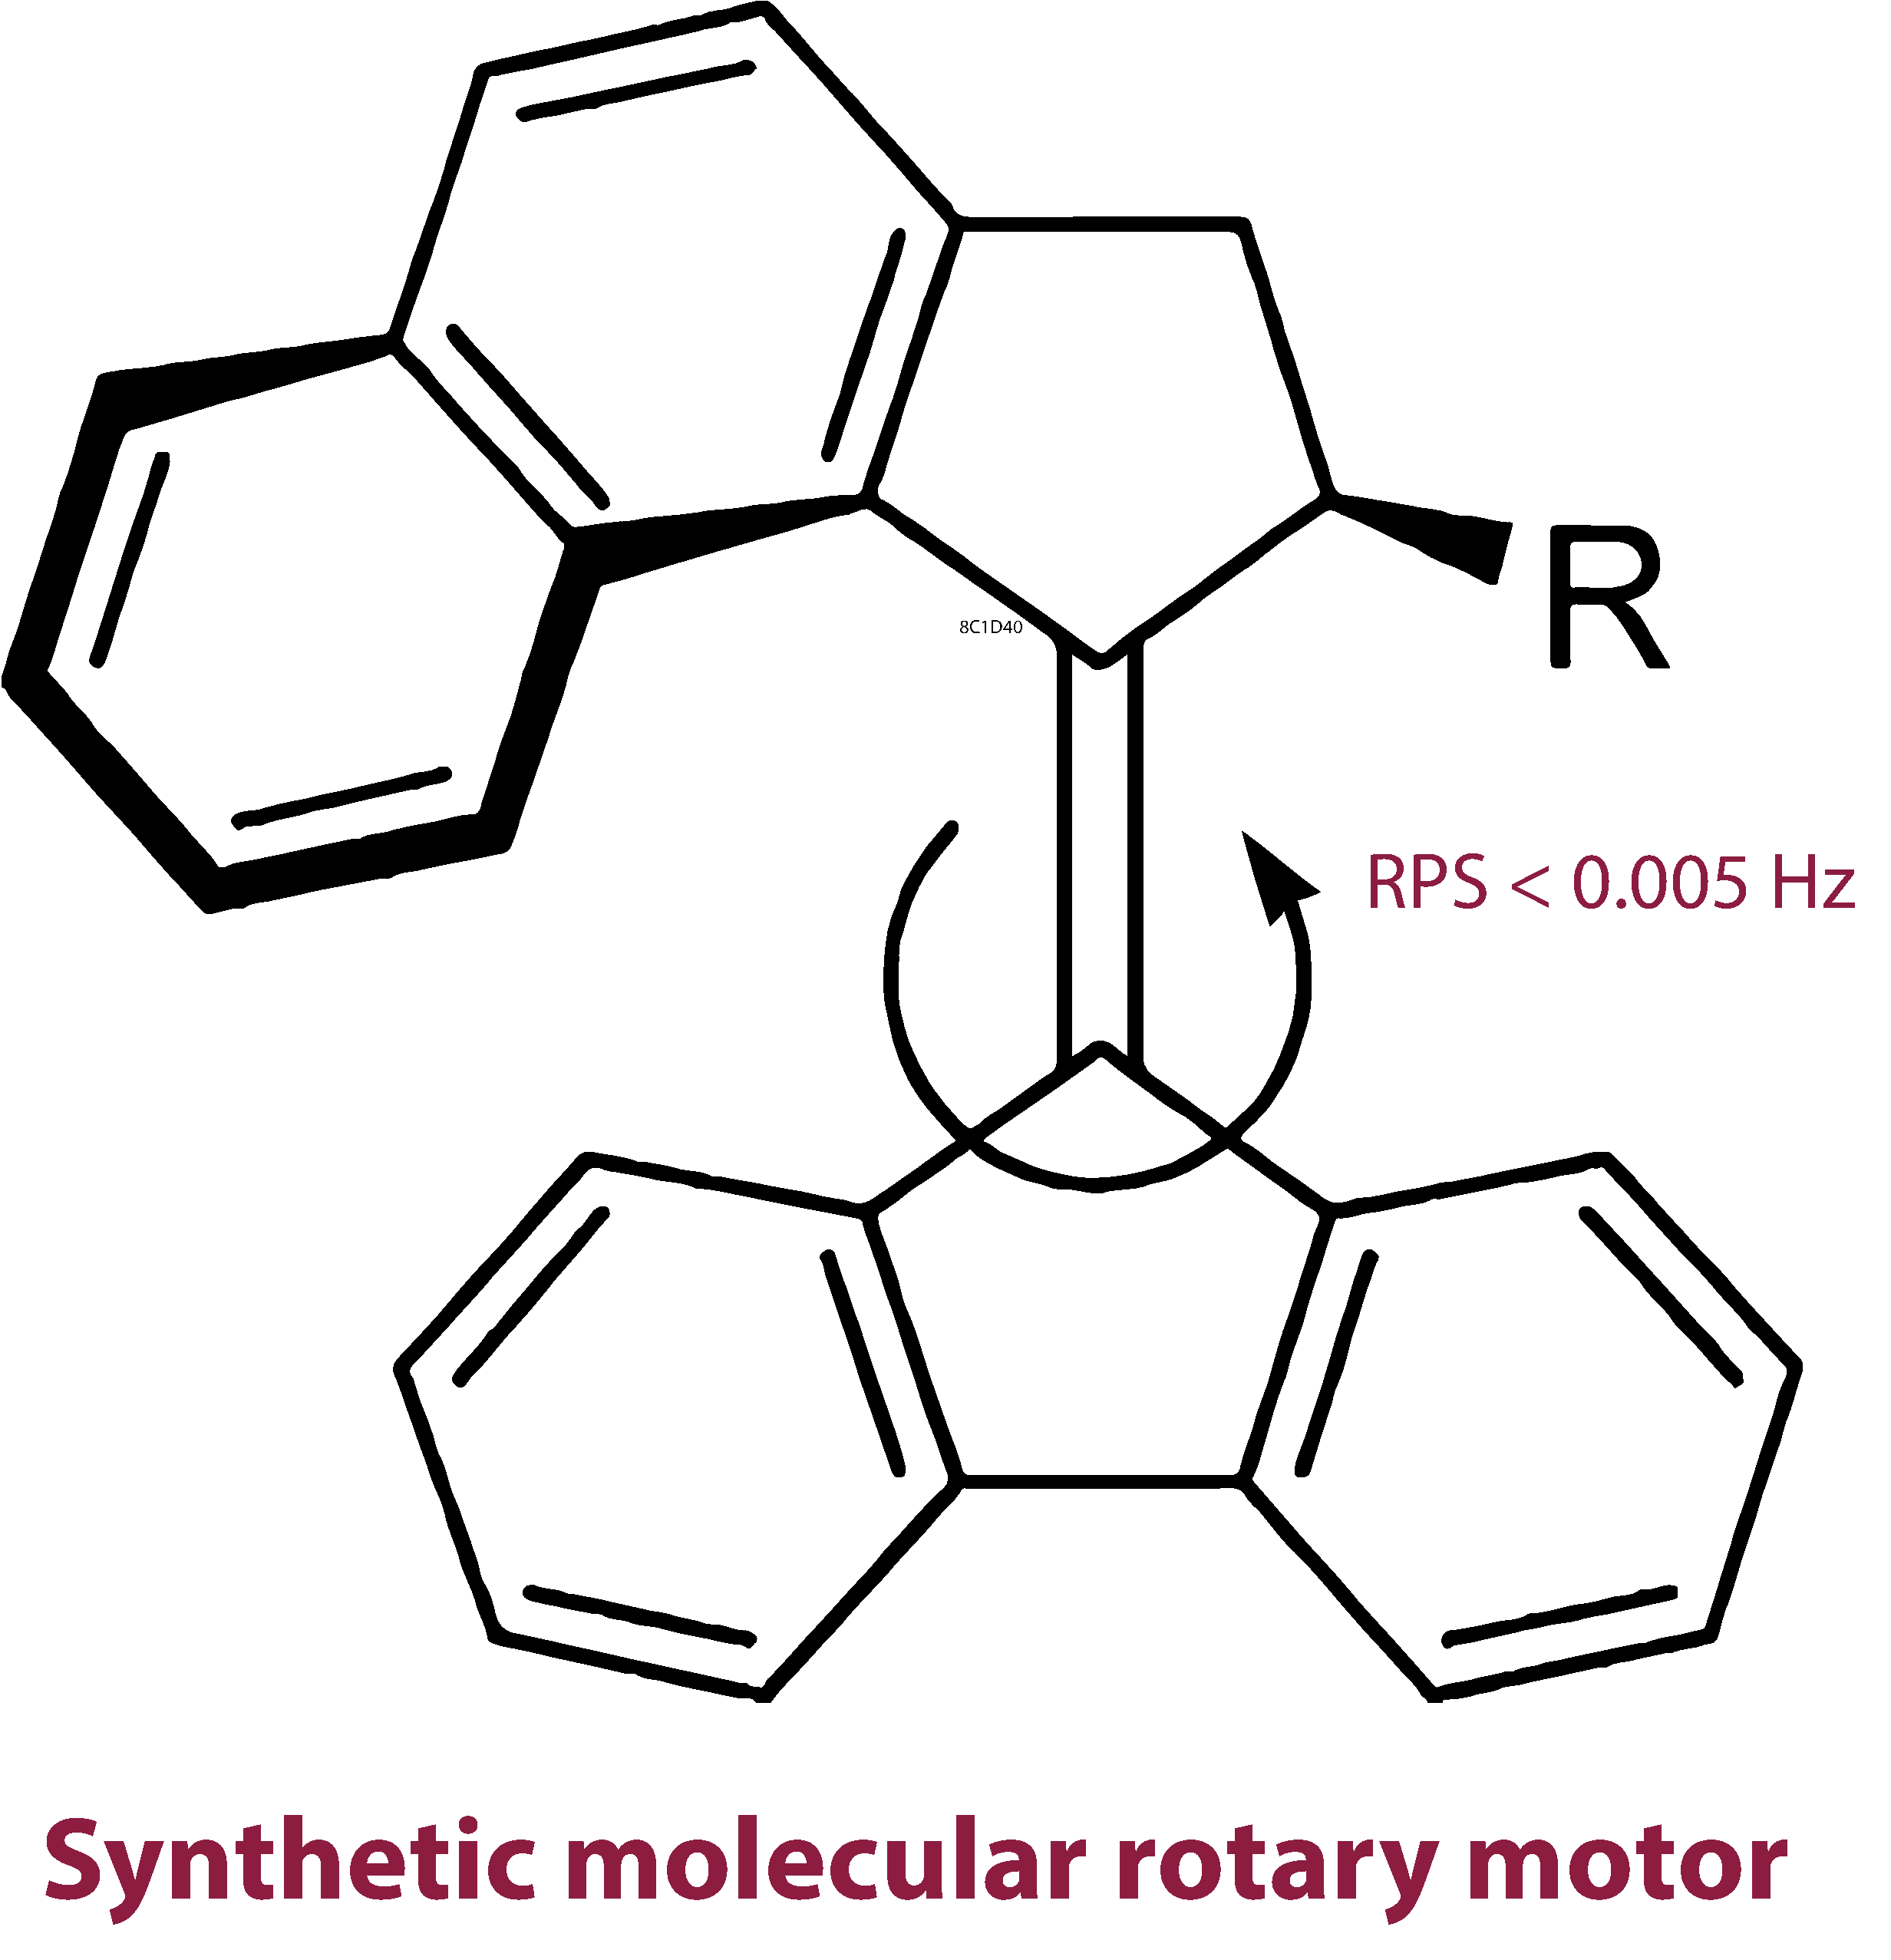
\includegraphics[width=0.9\textwidth]{./synthetic}
\end{figure}
\end{column}
\end{columns}

\vskip2.0ex
\item dsDNA may have a potential of becoming a molecular rotary motor \textbf{because of its helix shape}. Under a uniform field, the helix shape may generate a moment relative to the axis of dsDNA.

\item Broad implications: DNA nanopore sequencing, biosensing 

\end{enumerate}\vskip1.0ex
\end{block}\vskip0.5ex % }}}
\end{column}
%}}}

% ===== Column 2 ===== {{{
\begin{column}{.4\linewidth}\vskip -0.5ex

\begin{block}{Theoretical approach}
\vskip-2.5ex\begin{columns}
\hskip-1.6ex\begin{column}{.35\linewidth}
\begin{itemize}
\item Modeling dsDNA transversing through nanopore as circular channel flow with arbitrary height.
\end{itemize}
\end{column}
\begin{column}{.6\linewidth}
\vskip0.5ex\begin{center}\begin{figure}
	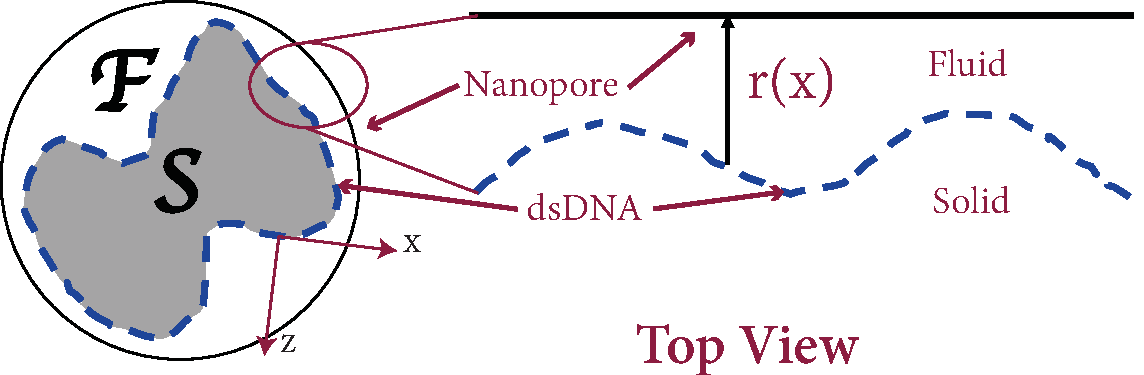
\includegraphics[width=0.99\textwidth]{problem_model}
\end{figure}\end{center}
\end{column}
\end{columns}
\vskip2.5ex

\begin{itemize}
\item Derived from Navier-Stokes equations:
	\begin{gather*}
    	\frac{d\rho}{dt} = 0 \quad\text{(mass)}	\quad\text{\textrm{\textit{\&}}}\quad\mu \mathbf{\nabla}^2 \mathbf{u} = \mathbf{\nabla}p + \text{\textbf{F}} \quad\text{(momentum)}
    \end{gather*}
\item Applying no-slip boundary conditions yields
\textcolor{asucrimson}{\begin{gather*}
    	\mathbf{u} = \frac{1}{2\mu} \left(\mathbf{\nabla}p - \mathbf{F}\right) z^2 - \left[\frac{1}{2\mu} \left(\mathbf{\nabla}p - \mathbf{F}\right)h^2 + \mathbf{U}\right] \frac{z}{h} + \mathbf{U}
    \end{gather*}}
\end{itemize}

\begin{columns}[t]
\hskip2.5ex
\begin{column}{.65\linewidth}
Parameterization for DNA shape by defining helix pitch constants:
\begin{gather*}
	k_x = \frac{2\pi}{L_{hp}} \quad\text{\textrm{\textit{\&}}}\quad k_y = -\frac{2\pi}{L_{hp} \tan{\theta}}
\end{gather*}
and minimum and maximum channel height:
\begin{gather*}
	h_0 = 0.5\text{nm} \quad\text{\textrm{\textit{\&}}}\quad h_1 = 1.35\text{nm}
\end{gather*}
yields:
\textcolor{asucrimson}{\begin{flalign*}
	\quad\qquad U_x =& -\frac{(h_1 - h_0)^2}{4(h_1 + h_0)} \left[\frac{k_x k_y}{\left(k_x^2 + k_y^2\right)}\right]\frac{F_y}{\mu} &\\
    &\left[\frac{1}{(h_1-h_0)} \ln{\left(\frac{h_1}{h_0}\right)}-\frac{2}{h_1+h_0}\right] \left(\frac{3k_x^2}{k_x^2+k_y^2}\right) &\\
    &+ \frac{1}{(h_1-h_0)}\ln{\left(\frac{h_1}{h_0}\right)} \Rightarrow \text{RPS} = \frac{Ux}{2\pi R}
\end{flalign*}} 
where $F_y$ can be related to voltage:
\begin{equation*}
	F_y = \frac{e V}{L_p}
\end{equation*}
\end{column}

\begin{column}{.35\linewidth}
\begin{center}\begin{figure}
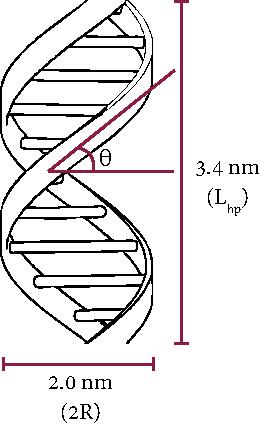
\includegraphics[width=0.98\textwidth]{./DNAModel}
\end{figure}\end{center}
\end{column}
\end{columns}

\begin{figure}
\includegraphics[width=0.98\textwidth]{./RPSData}
\end{figure}
\end{block}
\end{column}    
%}}}

% ===== Column 3 ===== {{{
\begin{column}{.28\linewidth}\vskip -0.5ex

\begin{block}{Experimental Setup} % {{{
\begin{itemize}
	\item A thin electrophoresis setup with two gold nanoparticles attached to the dsDNA
\end{itemize}\vskip1.0ex
\begin{figure}
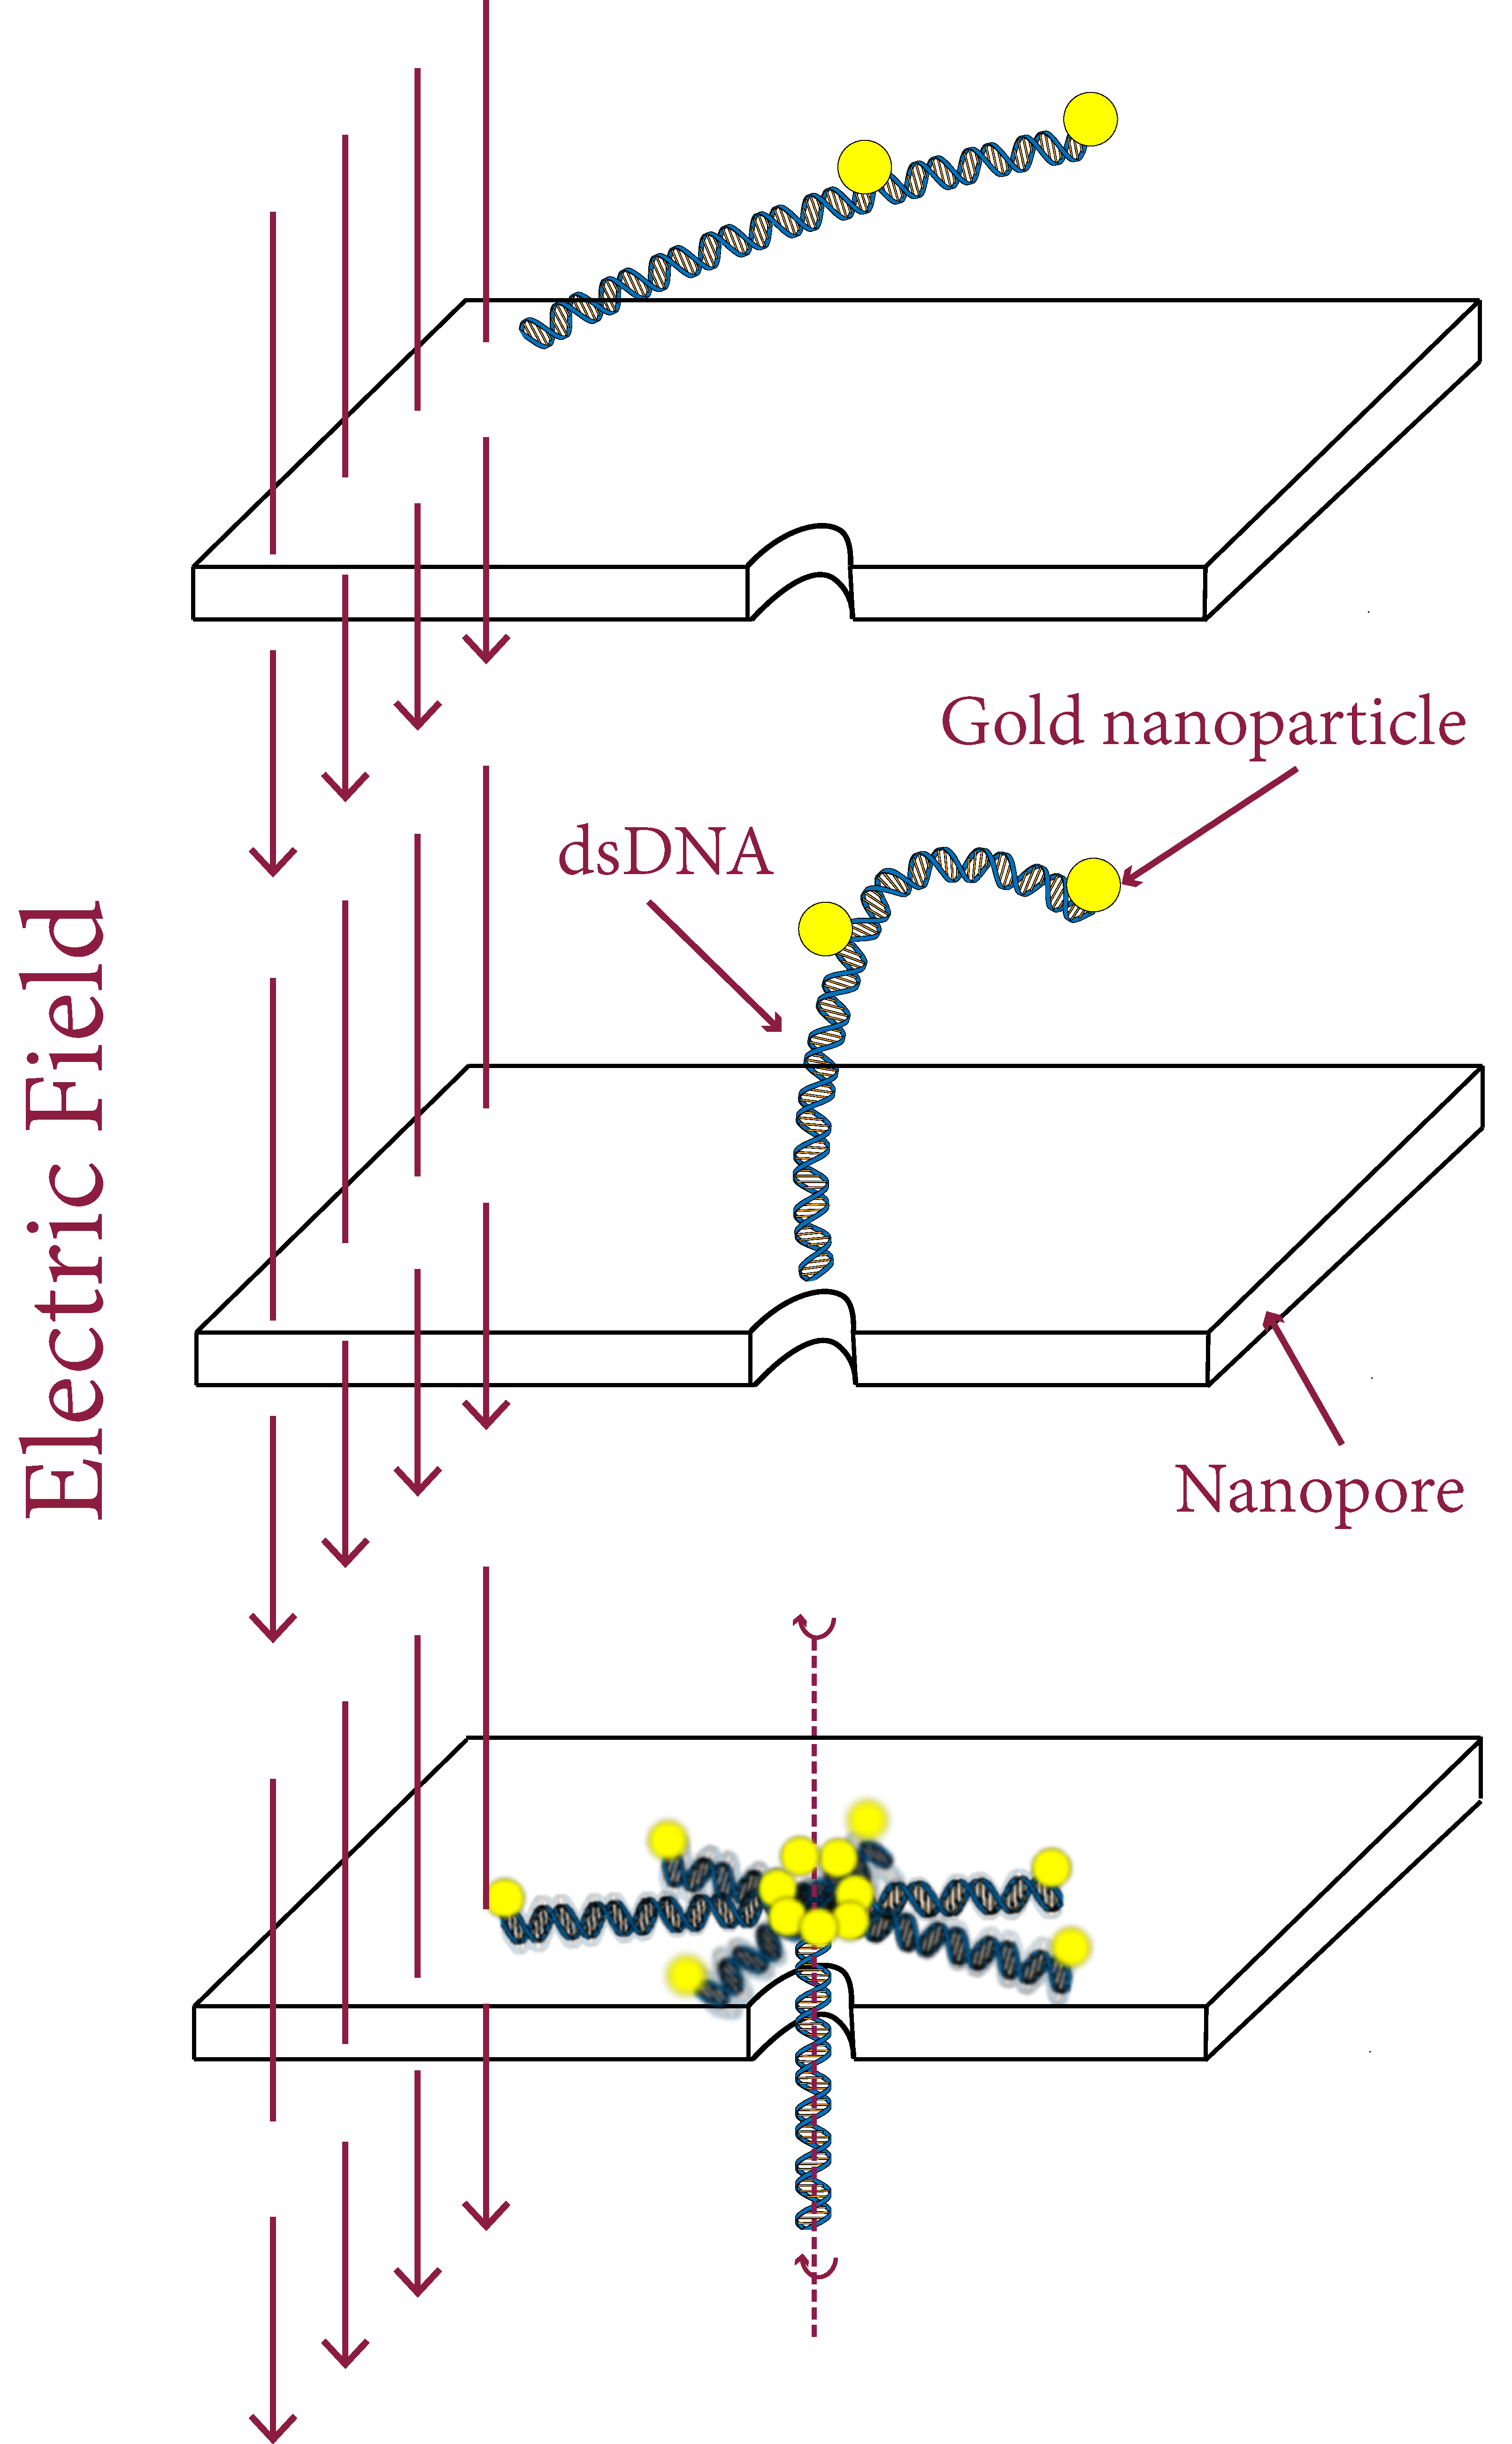
\includegraphics[width=0.75\textwidth]{./experiment}
\end{figure}
% \begin{itemize}
% 	\item A simple electrophoresis setup is built with small thickness to allow observation on microscope
% \end{itemize}\vskip1.0ex
% \begin{figure}
% 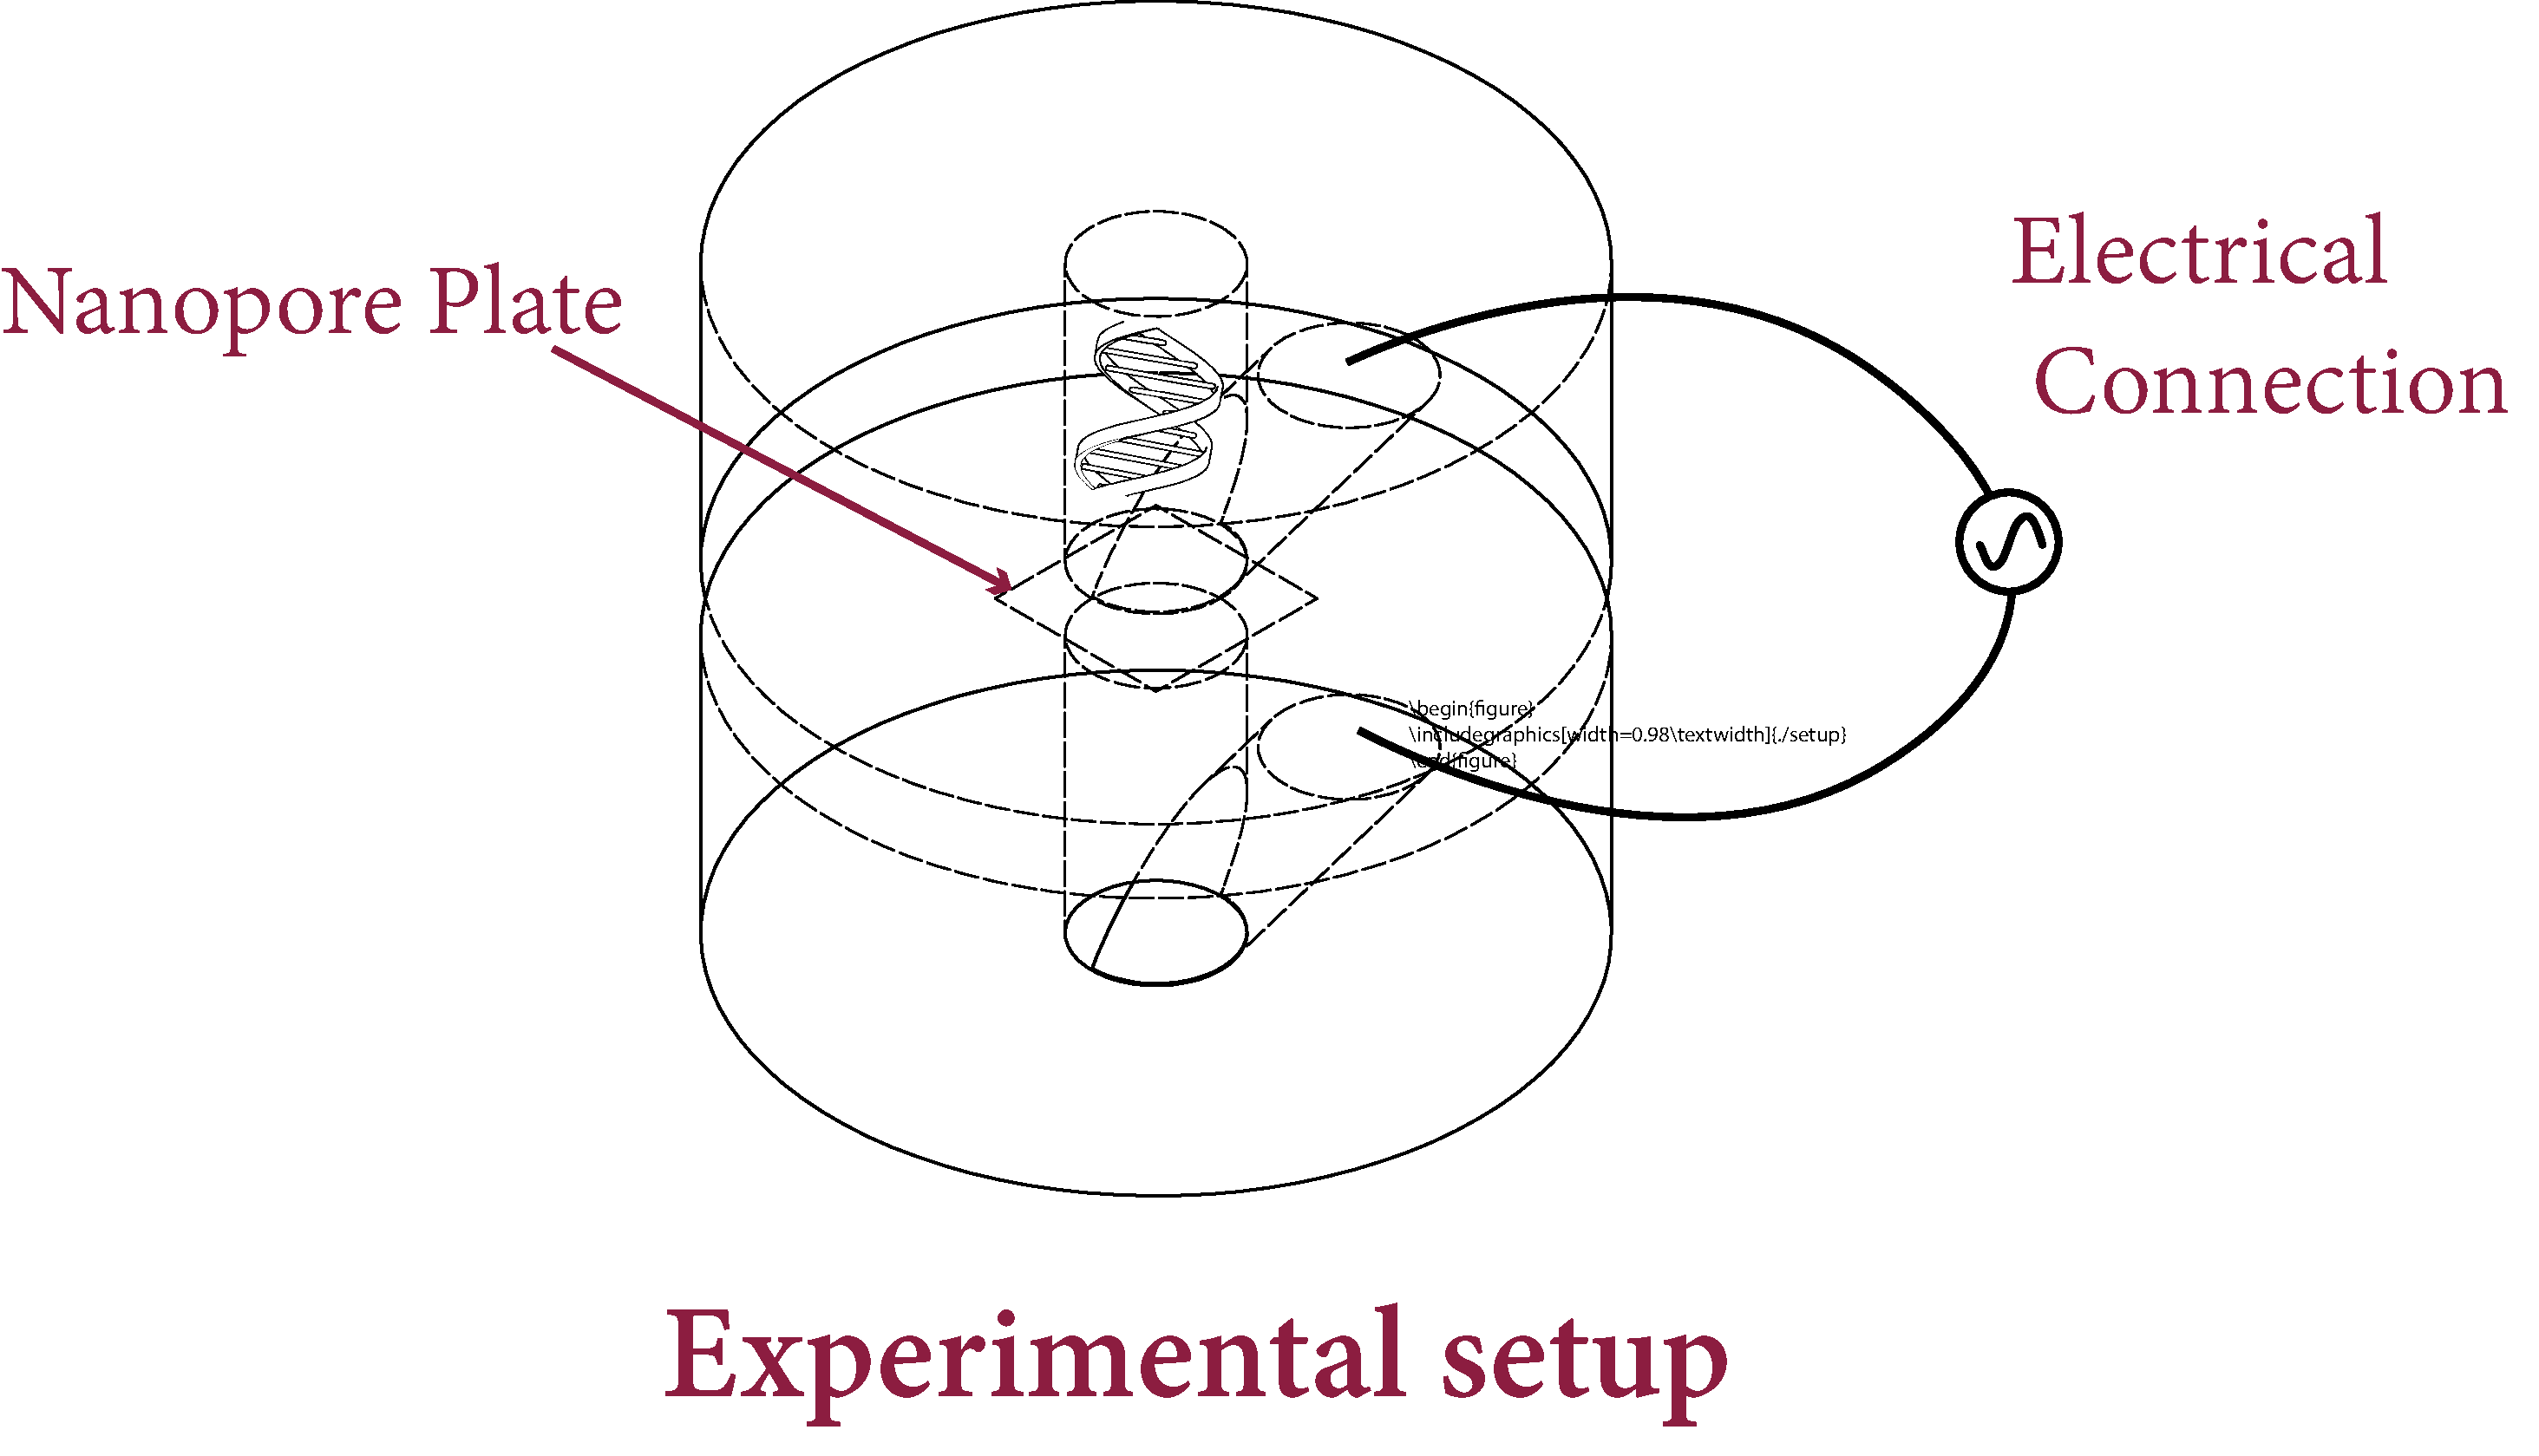
\includegraphics[width=0.75\textwidth]{./expsetup}
% \end{figure}
% 
% \begin{itemize}
% 	\item Two gold nanoparticles are attached to the edge of dsDNA allowing a clear detection of high speed rotation motion. The first gold nanoparticles will off-axis of dsDNA rotation as seen on the following figure.
% \end{itemize}\vskip0.5ex
% \begin{figure}
% 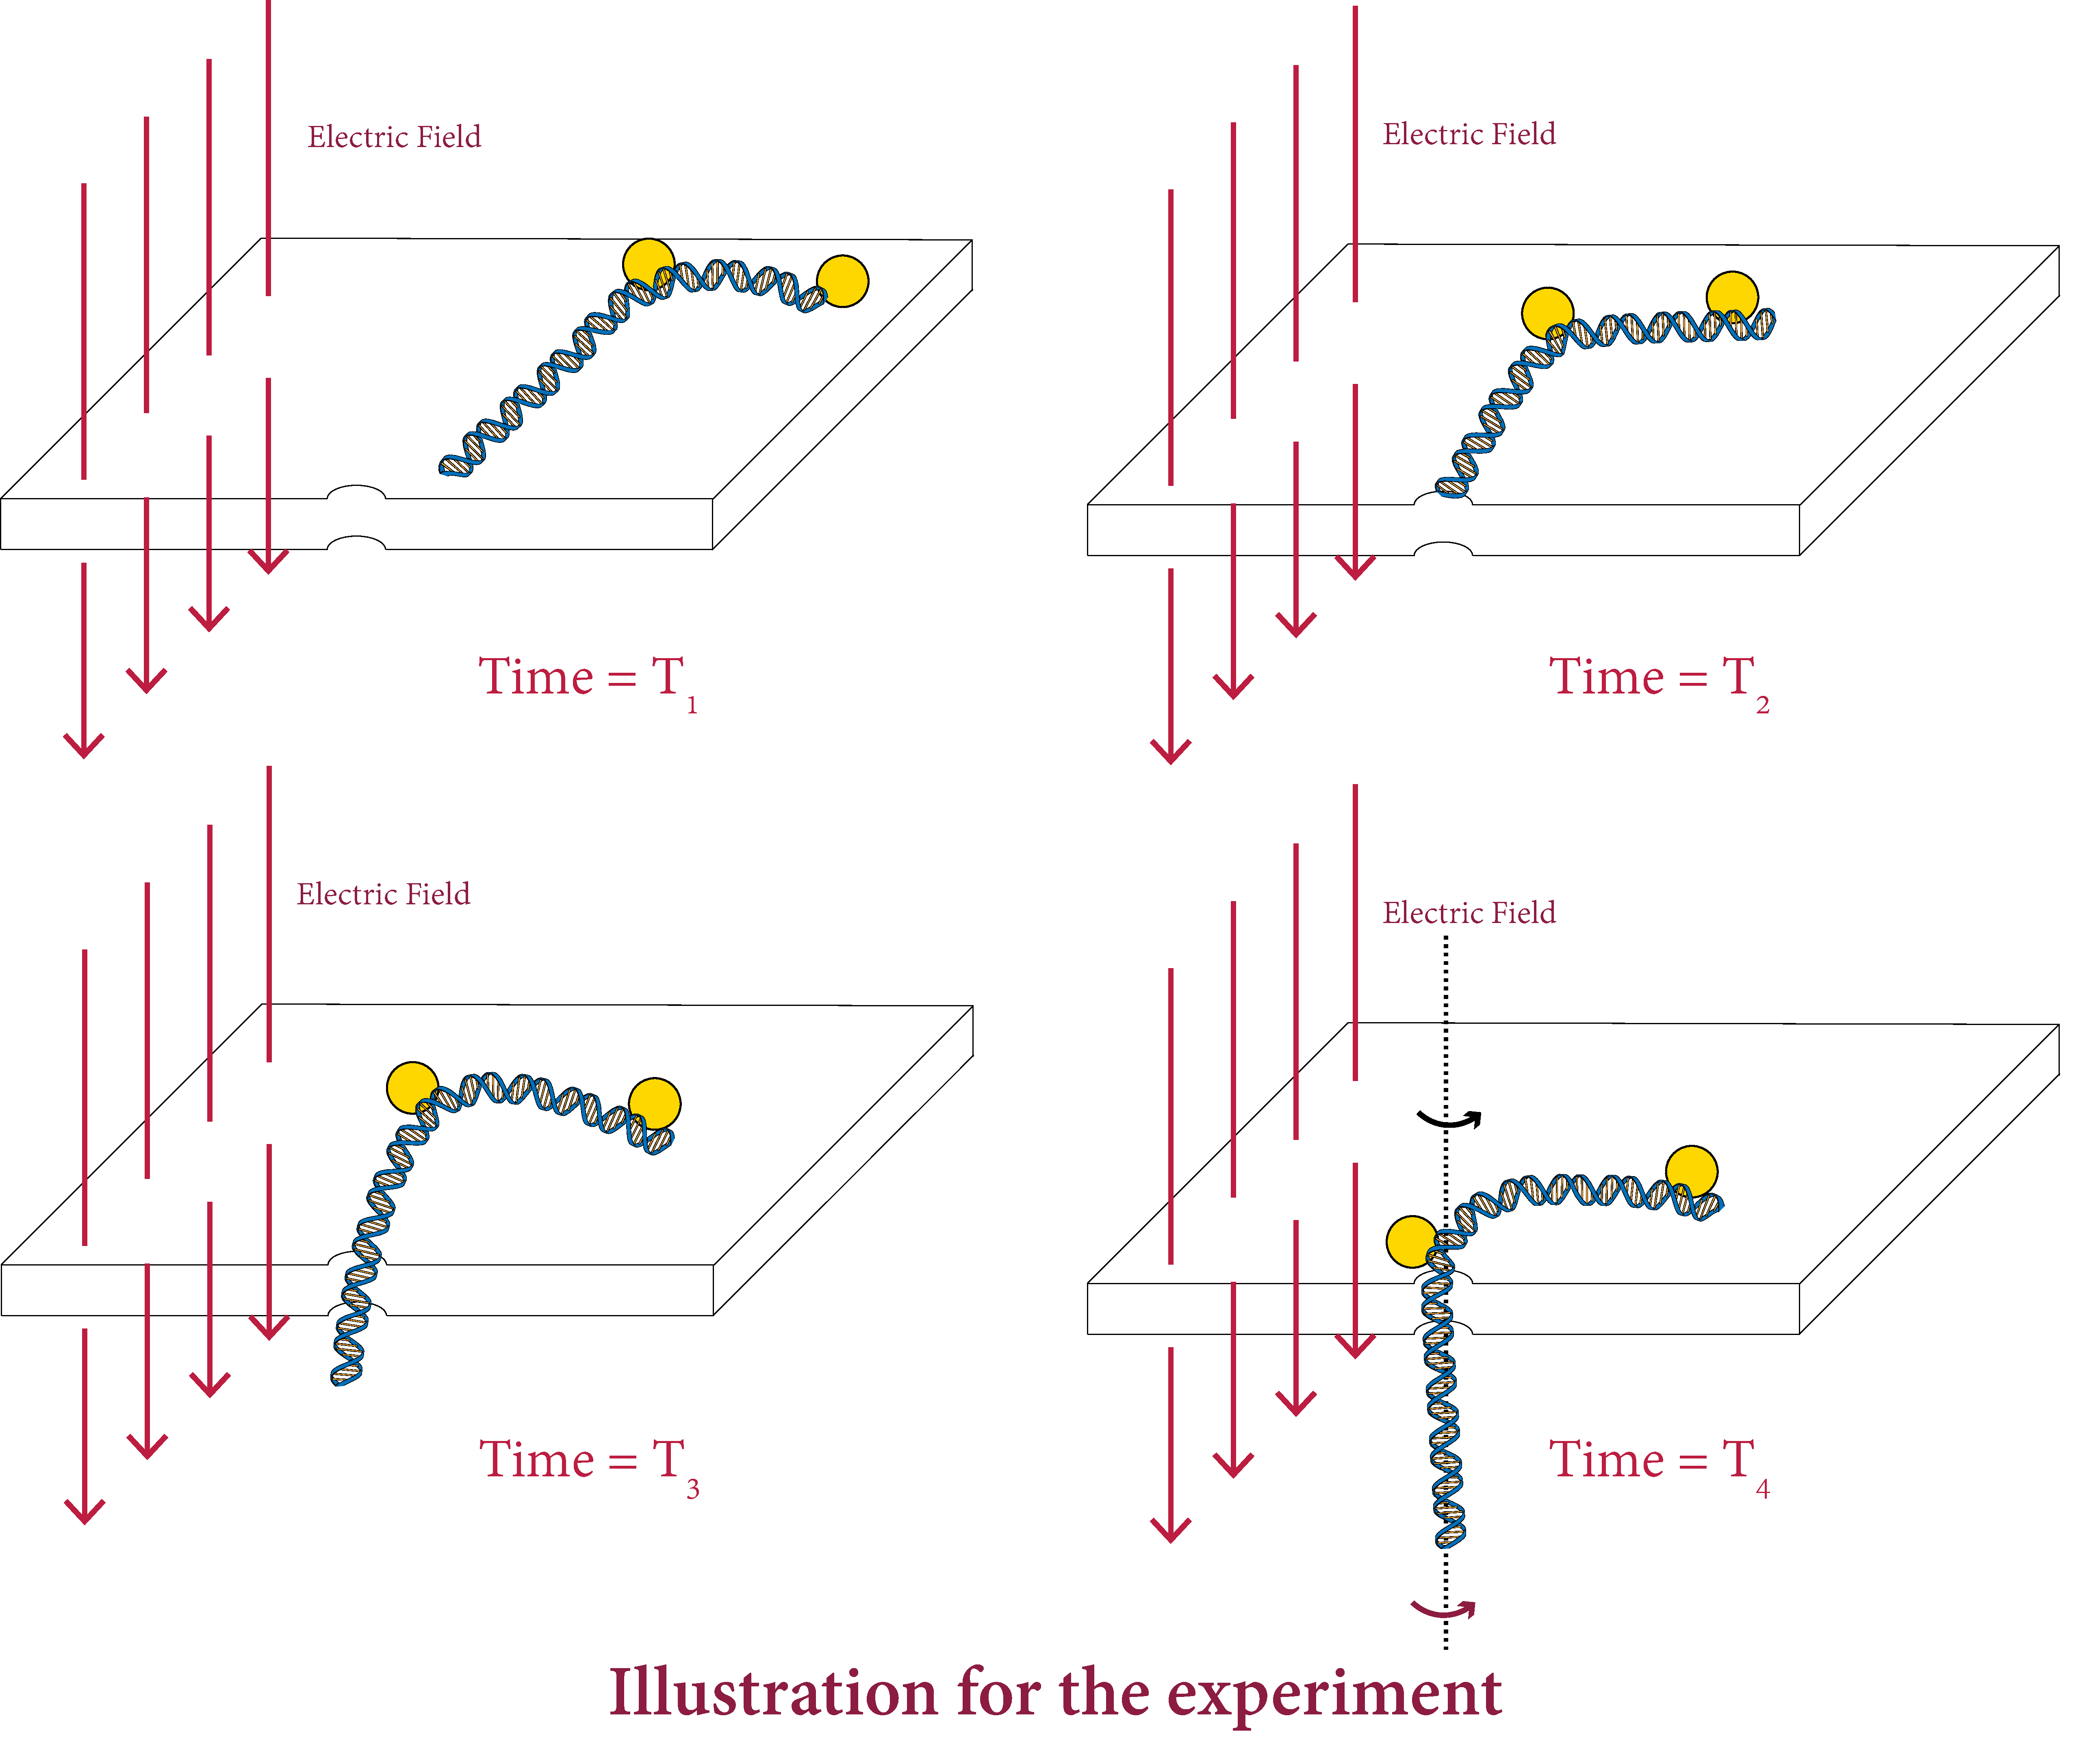
\includegraphics[width=0.98\textwidth]{./setup}
% \end{figure}
\end{block}\vskip2ex %}}}

\begin{block}{References} % {{{
\scriptsize 1. Serdyuk, Igor N., Nathan R. Zaccai, and Joseph Zaccai. Methods in molecular biophysics: structure, dynamics, function. , \textit{Cambridge University Press} 2007. \\
\scriptsize 2. Vicario, Javier, et al. "Fine tuning of the rotary motion by structural modification in light-driven unidirectional molecular motors." \textit{Journal of the American Chemical Society} 128.15 (2006): 5127-5135.
\end{block}\vskip2ex % }}}

\end{column}
%}}}

\end{columns}
\end{frame}

\end{document}
